\documentclass[twoside]{article}
\usepackage{exam}
\usepackage{enumitem}
\usepackage{verbatim}



\graphicspath{
    {figures/}
}

\pagestyle{myheadings}
\markboth{}{{\large Name: }\sp{4in}}
\nonstopmode

% For Python code
\lstset{%
  language=Python,
  basicstyle=\ttfamily,
  showstringspaces=false
  keywordstyle=\color{black},
  commentstyle=\color{black},
  stringstyle=\color{black},
}

\def\semester{Summer 2019}

\newcommand{\bubble}{\raisebox{-0.3ex}{
\includegraphics[height=2ex]{oval.png}}}
\newcommand{\filledbubble}{\raisebox{-0.3ex}{
\includegraphics[height=2ex]{oval-filled.png}}}
\newcommand{\lsi}{\lstinline}
\newcommand{\bkshort}{\underline{\qquad\qquad\qquad}\lsi}
\newcommand{\bk}{\underline{\qquad\qquad\qquad\qquad\qquad}\lsi}
\newcommand{\bkmed}{\underline{\qquad\qquad\qquad\qquad\qquad\qquad\qquad\qquad}\lsi}
\newcommand{\bklong}{\hrulefill}
\newcommand{\nlvs}{\newline\vskip 0.1in}

% Uncomment next line to generate pdf with solutions
%\newcommand{\issolution}{}

%%% Showing solutions %%%%%%%%%%%%%%%%%%%%%%%%%%%%%%%%%%%%%%%%%%%%%%%%%%%%%%%%%
\ifdef{\issolution}{%
    \newcommand{\solution}[1]{{\color{red}#1}}
    \newcommand{\solutioncircle}[1]{{\color{red}#1}}
    \newcommand{\solutionbubble}[0]{\filledbubble}
    \newcommand{\solutionimage}[2]{{\color{red}#2}}  % First arg is question, second is solution
    \newcommand{\versioned}[2]{{\color{red}#2}} % First arg is question, second is solution
}{%
    \newcommand\solution[1]{} % excludes
    \newcommand{\solutioncircle}[1]{#1} % don't color text but still display it
    \newcommand{\solutionbubble}[0]{\bubble}
    \newcommand{\solutionimage}[2]{#1} % First arg is question, second is solution
    \newcommand{\versioned}[2]{#1} % First arg is question, second is solution
}

\newcommand{\TBD}{{\color{red}{ TBD }}}

%%% Document %%%%%%%%%%%%%%%%%%%%%%%%%%%%%%%%%%%%%%%%%%%%%%%%%%%%%%%%%%%%%%%%%%

\title{\sc Midterm Exam \solution{Solutions}}

\begin{document}
\thispagestyle{empty}
\maketitle

\textbf{INSTRUCTIONS}

{\small
\begin{itemize}
\item The exam is worth 80 points. You have 110 minutes to complete it.

\item The exam is closed book, closed notes, closed computer/phone/tablet, closed calculator,
except the official midterm exam reference guide provided with the exam.

\item Write/mark your answers on the exam in the blanks/bubbles  provided. Answers written anywhere else will not be graded. Unless the question specifically asks you to explain your answer, you do not need to do so, and if you write an explanation it will not be graded.

\item If you need scratch paper, you are welcome to use the reference guide and the back of this cover page. Scratch work will not be graded.

\item For all Python code, you may assume that the statements \lstinline+from datascience import *+ and
\lstinline+import numpy as np+ have been executed.
Do not use features of the Python language that have not been described in this course.

\item In any part, you are free to use any tables, arrays, or functions that have been defined in previous parts of the same question, and you may assume they have been defined correctly.
\end{itemize}
}

\vskip .5in

\begin{center}
\begin{tabular}{|m{5.5cm}|m{8cm}|}
\hline
Last name & \\ [1cm]
\hline
First name & \\ [1cm]
\hline
Student ID number & \\ [1cm]
\hline
Calcentral email (\nolinkurl{\_@berkeley.edu}) & \\ [1cm]
\hline
Name of Lab GSI & \\ [1cm]
\hline
Your seat number (e.g. A1) \& room & \\ [1cm]
\hline
{\Large $\leftarrow$} Name of the person to your left & \\ [1cm]
\hline
Name of the person to your right {\Large $\rightarrow$} & \\ [1cm]
\hline
\emph{All the work on this exam is my own.} \textbf{(please sign)} & \\ [1cm]
\hline
\end{tabular}
\end{center}

\clearpage
\textbf{This page is intentionally left blank. You can use it for scratch work but it will not be graded.}
~\newpage

\begin{enumerate}
      \q{22}{Get Off Your Phone}
\vskip .2in

A digital media company commissions a Berkeley Data Science club to conduct an analysis about how much time people spend on their phones. The club surveyed 500 people and collected the resulting data in the table \lsi+phones+ which has 5 columns: 
\begin{itemize}
    \item \lsi+Name+: The person's name
    \item \lsi+Model+: The type of phone the person has, an 'iPhone', 'Samsung Galaxy', 'Google Pixel', or 'Non-smartphone'
    \item \lsi+Screentime+: The average daily minutes that person spends on their phone
    \item \lsi+Data (MB/day)+: The average daily cell data usage of that person, in megabytes
    \item \lsi+Provider+: The person's cell phone carrier: 'AT\&T', 'Verizon', 'Sprint', or 'T-Mobile'
\end{itemize}

Here are the first 5 rows of the table, which has 500 rows total:
\begin{center}
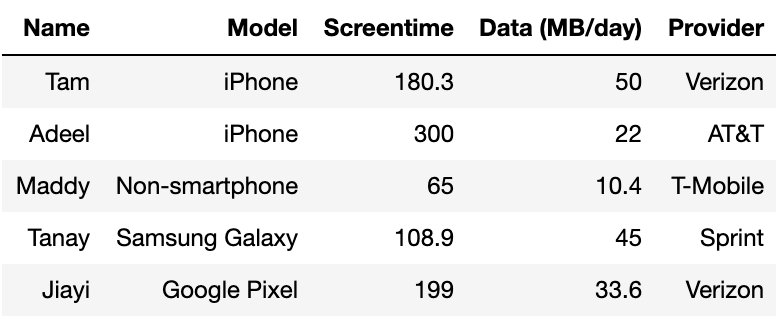
\includegraphics[scale=.9]{q1_phones}
\end{center}
\vskip .1in
\textbf{Fill in the blanks with Python expressions to compute the desired output.} ONLY use the blank lines provided. Some of the chained operations we might normally do in one line have been broken up into two or more lines,
storing intermediate results in tables or arrays. Do not write any code outside the blanks provided. The
expression in the last line should evaluate to the value described in the question.

\begin{enumerate}
\vskip 0.2in
\subq{2} Write code to assign \lsi+least_screen+ to the smallest value of daily screentime in the \lsi+phones+ table.
\vskip .2in
\solutionimage
{
\lstinline+least_screen =+\bklong\newline
}
{
\lstinline+least_screen = min(phones.column("Screentime"))+
}


\subq{3} Write code that assigns \lsi+num_iphones+ to the number of people with iPhones in the \lsi+phones+ table. 
\vskip .2in
\solutionimage
{{\lsi+iphones = phones.+\bkshort+("Model",+\bk+(+\bk+)+\nlvs}
\lstinline+num_iphones = iphones.+\bkmed
}
{
\lsi+iphones = phones.where("Model", are.equal_to("iPhone"))+\newline
\lstinline+num_iphones = iphones.num_rows+
}



\vskip .2in
\subq{4} Write code that assigns \lsi+high_provider+ to the cell phone provider of the person with the highest data usage. You can assume that data usages are unique in the \lsi+phones+ table.

\solutionimage
{
\vskip .2in
{\lsi+sorted = phones.+\bkshort+(+\bk+,+\bkmed+)+\nlvs}
{\lsi+high_provider = sorted.+\bkshort+.(+\bk+).+\bkshort+(+\bk+)+\nlvs}
}
{
\vskip .2in
\lsi+sorted = phones.sort("Data MB/day", descending=True)+\newline
\lstinline+high_provider = sorted.column("Provider").item(0)+
\vskip .4in
}




\subq{3} Write code that assigns \lsi+average+ to a table with two columns: one containing all of the phone models, and another containing the average screentime for each model.
\vskip .2in
\solutionimage
{
{\lsi+average = phones.+\bkshort+(+\bkshort+,+\bkshort+).select(+\bkshort+,+\bk+)+\nlvs}
}
{
\lsi+average = phones.group("Model", np.mean).select("Model", "Screentime mean")+
\vskip 0.2in
}


\subq{6} Later on in the project, a club member creates a table with information about cell phone providers and data costs. The \lsi+providers+ table has two columns:
\begin{itemize}
    \item \lsi+Company+: The name of the cell phone provider (“AT\&T”, “Verizon”, “Sprint”, or “T-Mobile”)
    \item \lsi+Price ($/MB)+: The price the company charges per megabyte of data used.
\end{itemize}
\begin{center}
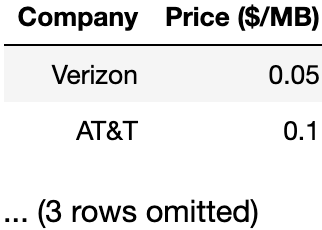
\includegraphics[scale=1]{q1_providers}
\end{center}
Write code to generate a table called \lsi+costs+ which contains two columns:
\begin{itemize}
    \item \lsi+Name+: The name of the person in the study
    \item \lsi+Monthly Cost+: The price the person has to pay for 30 days of data usage. Assume that every day, the person used the usage amount listed in the \lsi+phones+ table.
\end{itemize}
\vskip 0.2in
\solutionimage
{
{\lsi+all_info = phones.+\bkshort+(+\bk+,+\bk+,+\bk+)+\nlvs}
%{\lsi+daily_cost = +\bkshort+.+\bkshort+(+\bkshort+) * +\bkshort+.+\bkshort+(+\bkshort+)+\nlvs} %FIXME these lines r gonna be too short, probs need to split across lines
{\lsi+daily_usage = +\bkshort+.+\bk+(+\bk+)+\nlvs}
{\lsi+prices = +\bkshort+.+\bk+(+\bk+)+\nlvs}
{\lsi+daily_cost = daily_usage * prices +\nlvs}

{\lsi+monthly_cost = daily_cost * 30+\nlvs}
{\lsi+costs = Table().+\bk+(+\nlvs}
\hspace{1in}{\lsi+'Name', +\bkmed+,+\nlvs}
\hspace{1in}{\lsi+'Monthly Cost', +\bkmed+)+\nlvs}
}
{
{\lsi+all_info = phones.join("Provider",providers,"Company")+\nlvs}
%{\lsi+daily_cost = +\bkshort+.+\bkshort+(+\bkshort+) * +\bkshort+.+\bkshort+(+\bkshort+)+\nlvs} %FIXME these lines r gonna be too short, probs need to split across lines
{\lsi+daily_usage = all_info.column("Data MB/day")+\nlvs}
{\lsi+prices = all_info.column("Price $/MB")+\nlvs}
{\lsi+daily_cost = daily_usage * prices +\nlvs}

{\lsi+monthly_cost = daily_cost * 30+\nlvs}
{\lsi+costs = Table().with_columns(+\nlvs}
\hspace{1in}{\lsi+'Name', all_info.column("Name"),+\nlvs}
\hspace{1in}{\lsi+'Monthly Cost', monthly_cost)+\nlvs}
}

\vskip 2in

\subq{2} Write code so that \lsi+summary+ results in the following table:
\begin{center}
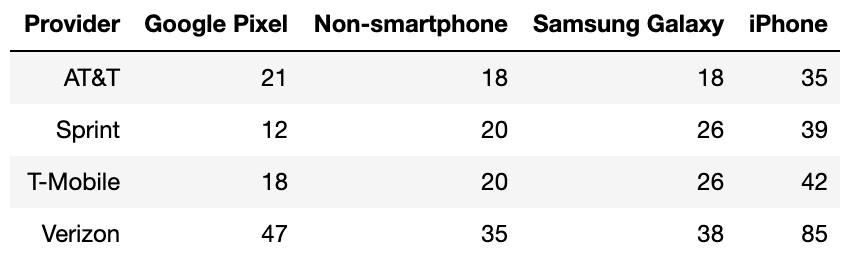
\includegraphics[scale=1]{q1_pivot}
\end{center}
The value in each cell represents the number of  people in the survey that had the corresponding phone/provider combination.
\vskip .1in
\solutionimage
{
\lstinline+summary = phones.+\bklong\newline
}
{
\lstinline+summary = phones.pivot("Model", "Provider")+
}

\vskip .3in
\subq{2} The following is a plot displaying the count of each phone model in the \lsi+phones+ table:
\begin{center}
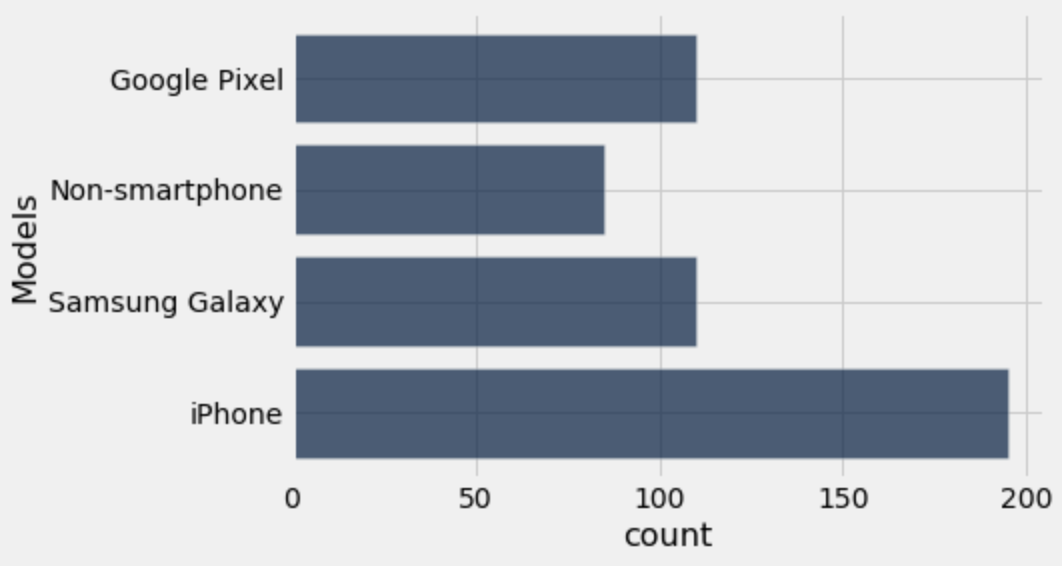
\includegraphics[scale=0.5]{q1_models}
\end{center}
Which line of code generated the above plot? 
\vskip .1in
{\bubble} \lsi+phones.barh('Model')+ \\
\solutionimage{\bubble}{\filledbubble}\lsi+phones.group('Model').barh('Model')+ \\
{\bubble} \lsi+phones.hist('Model')+\\
{\bubble} \lsi+phones.group('Model').hist('Model')+\\

\end{enumerate}

      \clearpage
      \q{8}{Street Smarts}
\vskip .1in
In 2015, economists Melissa Kearney and Phillip Levine published a study investigating the effects of watching \textit{Sesame Street} on the future academic performance of young viewers in the early 1970s. \textit{Sesame Street} is a popular children’s show that was first introduced in 1969 and provides free educational content on public television to children who are too young to attend school.
\vskip .2in
However, there was variation in exposure to \textit{Sesame Street} across the country, due to technological constraints. Approximately 1/3 of US viewers lived in counties where they were unlikely to be able to view \textit{Sesame Street}. Whether or not a county had high rates of access to \textit{Sesame Street} was close to random and was not associated with any particular characteristics of the county, such as income.
\vskip .2in
Since the researchers did not have data on whether individual children watched \textit{Sesame Street}, they instead investigated county-level elementary-school success metrics of groups of children who started school after the show debuted and who lived in locations where broadcast reception for the show was high, and compared these metrics to those among older groups of children (who would not have watched \textit{Sesame Street} before starting school) and those who lived in locations with limited broadcast reception (poor likelihood of access to \textit{Sesame Street}). 
\vskip .2in
The authors found that "children who lived in places with better access to the show did better [on average] in elementary school, as compared to those with limited access and those who were older at the time the show was introduced. They were more likely to start school on time and progress at the appropriate grade for age."
\begin{enumerate}
\vskip .3in
\subq{2} Who were the individuals in this study?\vskip 0.1in


{\bubble} Individual children who started school after \textit{Sesame Street} debuted in the United States\\[2pt]
{\bubble} Individual children who started school just before or after \textit{Sesame Street} debuted in the United States\\[2pt]
\solutionimage{\bubble}{\filledbubble}  Groups of children in different counties in the United States\\[2pt]
{\bubble}  Groups of children in different counties with high likelihood of access to \textit{Sesame Street} in the United States


\vskip .25in
\subq{2} The authors made two comparisons:\vskip 0.1in
\begin{itemize}
\item They compared the educational outcomes of groups of children in counties with high likelihood of access to \textit{Sesame Street} to the educational outcomes of groups of children with low likelihood of access to \textit{Sesame Street}.
\item They compared the educational outcomes of groups of children in counties with high access to \textit{Sesame Street}, and who started school after \textit{Sesame Street} debuted, to groups of children \textbf{in those same high-access counties} who started school before \textit{Sesame Street} debuted on television.
\end{itemize}
\vskip 0.1in
Why did the authors include both comparisons in their study?

{\bubble} The authors thought children may have moved from one county to another, so they wanted to study the children who moved by looking at the same group over time.\\[4pt]
{\bubble} By studying the same children before and after they watched \textit{Sesame Street}, the authors could determine whether \textit{Sesame Street} was the reason that some individual students performed better than others.\\[4pt]
{\bubble}  The authors wanted to include more children in their study (a larger sample size) so that the children would be more representative of the population of all children in the United States, instead of just looking at one age group.\\[4pt]
\solutionimage{\bubble}{\filledbubble}  Making both comparisons helps eliminate the possibility of confounding factors due to broadcast variability (which counties had \textit{Sesame Street} access) or variation in educational quality across years (if education in general improved or got worse over the study period).

\vskip .4in
\subq{4} Select \textbf{all} correct statements:\vskip 0.1in


\solutionimage{\bubble}{\filledbubble} This was an observational study.\\[2pt]
{\bubble} This was a randomized controlled experiment.\\[2pt]
{\bubble} It is only possible to investigate a causal link with a randomized controlled experiment, and this study did not help establish a causal link between \textit{Sesame Street} and better educational outcomes.\\[2pt]
{\bubble} Whether or not a child lived somewhere with access to \textit{Sesame Street} was random, \\because the researchers split the groups of children into a treatment and a control group.\\[2pt]
\solutionimage{\bubble}{\filledbubble}  The authors were attempting to use a natural experiment, the variation in TV signals, \\to establish a causal link between watching \textit{Sesame Street} and better educational outcomes.\\[2pt]


\end{enumerate}
      \clearpage
      \q{12}{Boba Distributions}

Anna is curious about her boba spending habits. The following is a histogram of her weekly spending on boba, over the span of \textbf{50} weeks (she doesn’t drink boba on her yearly two week vacation): 
%FIXME Do we like placement of hist? 
\begin{center}
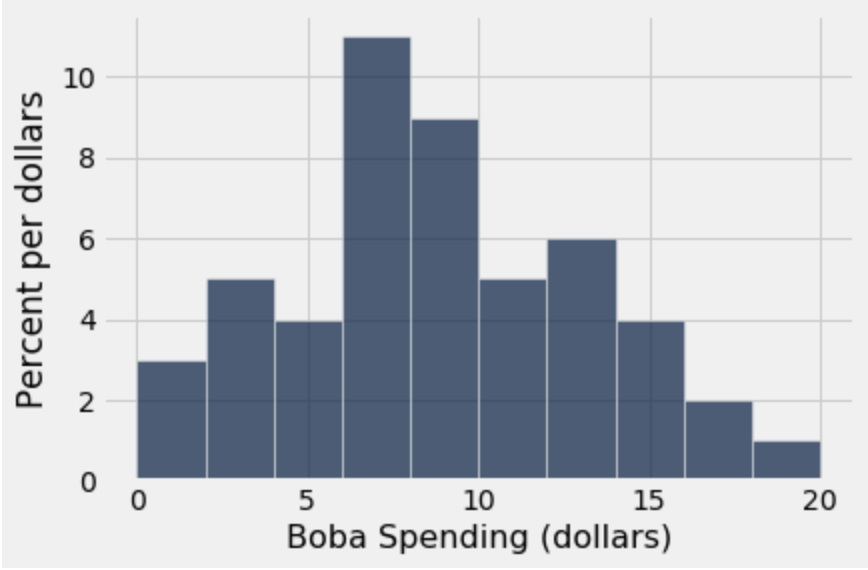
\includegraphics[scale=.6]{q3_boba}
\end{center}
The spending is divided into bins of width 2: [0,2), [2,4) ... [18,20).  

Assume that all of the data is shown on the histogram (Anna never spent \$20 or more in a given week).  

For the following questions, write a \textbf{mathematical expression} for the answer, or write \textit{“Not possible”} if it is not possible to calculate the desired quantity with the information in the given histogram.

\begin{enumerate}
\vskip .2in
% Do we want to bold percent? 
\subq{3} In what percent of weeks did Anna spend \$16 or more on boba?

\solution{2*2 + 1*2 = 6\%}

\vskip .6in
% Do we want to bold percent? 
\subq{3} In what percent of weeks did Anna spend between \$12 and \$15 on boba? 

\solution{Not possible to determine}

\vskip .6in
\subq{3} During how many weeks did Anna spend between \$10 and \$13 dollars?

\vskip 0.1in
\begin{tabular}{l@{\hskip 1in}l@{\hskip 1in}l@{\hskip 1in}l}
\bubble\quad 11 weeks \\
\solutionbubble \quad Between 5 and 11 weeks \\
\bubble \quad 22 weeks \\
\bubble \quad Between 10 and 22 weeks \\
\bubble \quad Not possible to calculate using the histogram
\end{tabular}

\vskip .2in
\subq{3} After looking over her notes, Anna finds that she entered the wrong data for two of the weeks when constructing the histogram. She is not sure whether her spending in those weeks should go in the [12, 14) or [14, 16) bin, so she decides to combine all of the data in those two bins into one bin of width 4, from [12,16). What is the height of this new bin? 

\solution{(0.6*2 + 0.4*2)/4 = 5 \%/\$}


\end{enumerate}

      \clearpage
      \q{10}{Steph Curry Fan Club}

A group of current Data 8 students who are big fans of Steph Curry are inspired by the current course material to conduct an analysis of Curry's basketball shot record. It turns out Steph Curry has a 58\% chance of successfully shooting the ball in the basket any time he tries. 



\begin{enumerate}
\vskip .2in
\subq{2} Curry shoots the ball twice. What is the probability that both of the shots make it in the basket?\vskip 0.1in
\begin{tabular}{l@{\hskip 1in}l@{\hskip 1in}l@{\hskip 1in}l}
{\bubble} \quad ${\displaystyle \frac{58}{100}\times \frac{58}{99}}$
&\solutionbubble \quad ${\displaystyle 0.58^2}$ \\[10pt]
\bubble \quad ${\displaystyle 2 \times 0.58 }$
&\bubble \quad ${\displaystyle 0.42^2}$

\end{tabular}


\vskip .4in
\subq{2} Curry shoots the ball twice. What is the probability that one shot makes it into the basket, and one shot does not?\vskip 0.1in

\begin{tabular}{l@{\hskip 1in}l@{\hskip 1in}l@{\hskip 1in}l}
{\bubble}\quad ${\displaystyle (0.58\times0.42)^2 }$
&\bubble \quad  ${\displaystyle 0.58 \times 0.42 }$ \\[10pt]
\solutionbubble \quad  ${\displaystyle (0.58\times0.42) + (0.42\times0.58)}$
&\bubble \quad ${\displaystyle 1 - (0.58)^2 }$
\end{tabular}
\end{enumerate}


\begin{enumerate}[resume]
\vskip .4in
Digging deeper into Steph Curry's basketball record, the students find that 80\% of Curry’s shots are contested - that is, someone is actively trying to block his shot or make him miss. When a shot is contested, Curry has a 55\% chance of successfully shooting the ball in the basket any time he tries. When his shots are not contested, Curry has a 70\% chance of shooting the ball in the basket. 



\vskip.4in
\subq{2} Given that Steph Curry's shot was uncontested, what is the probability the shot did not make it in the basket?\vskip 0.1in

\begin{tabular}{l@{\hskip 1in}l@{\hskip 1in}l@{\hskip 1in}l}
{\bubble}\quad ${\displaystyle \frac{0.2\times0.3 }{(0.2\times0.3 + 0.8\times0.45)}}$
&\bubble \quad  0.42 \\[12pt]
\solutionbubble \quad  0.30
&\bubble \quad ${\displaystyle (0.2\times0.3) + (0.8\times0.45) }$
\end{tabular}



\vskip .4in
\subq{2} Given that Steph Curry took three contested shots in a row, what is the probability that at least one of them went in?\vskip 0.1in

\begin{tabular}{l@{\hskip 1in}l@{\hskip 1in}l}
\solutionbubble \quad ${\displaystyle 1 - (0.45)^3}$
&\bubble \quad  ${\displaystyle 1 - (3\times0.45) }$ \\[10pt]
\bubble \quad  ${\displaystyle \frac{0.80\times0.55}{[(0.80\times0.55) + (0.20\times0.70)]^3}}$
&\bubble \quad ${\displaystyle 0.55^3 }$
\end{tabular}



\vskip .4in
\subq{2} Given that Steph Curry made the shot, what is the probability the shot was contested?\\

\begin{tabular}{l@{\hskip 1in}l@{\hskip 1in}l@{\hskip 1in}l}
{\bubble} \quad ${\displaystyle \frac{0.20\times0.70}{\big((0.80\times0.55) + (0.20\times 0.70)\big)}}$
&\bubble \quad  ${\displaystyle 1 - (0.45)^3}$\\[10pt]
\bubble \quad 0.8
&\solutionbubble \quad  ${\displaystyle \frac{0.80\times0.55}{\big((0.80\times0.55) + (0.20\times0.70)\big)}}$
\end{tabular}

\end{enumerate}


      \clearpage
      \q{28}{Issues with Influenza}

The national news reports widespread hospitalizations from flu this year in the United States. Since you don't remember the media reporting on this in the past, you want to know if this year's incidence rate of flu (the proportion of the population who become infected with influenza) in the U.S. is higher than usual. Since you only have the resources to take a random survey of 1000 people, you decide to conduct a hypothesis test to find out.

After conducting your random survey of 1000 people, you find that the incidence rate among this sample is 0.35. In modern history (since the invention of the influenza vaccine), the expected incidence rate is 0.2.
\begin{enumerate} 
    \subq{3} What is the appropriate null hypothesis?
    \vskip 0.05in
    {\bubble} Our sample is large enough to represent the US population.\\[2pt]
    {\bubble} The true incidence rate is 0.35, and 0.2 is an inaccurate estimate of historical incidence rates.\\[2pt]
    {\bubble} The true incidence rate of influenza this year is greater than 0.2, and our survey incidence rate is representative of the true incidence rate.\\[2pt]
    {\solutionbubble} The true incidence rate of influenza this year is 0.2, and any deviation from this rate is due to chance in the selection of the random sample.\\[2pt]

    \subq{3} What is the appropriate alternative hypothesis?
    \vskip 0.05in
    {\bubble} Our sample was not representative of the US population.\\[2pt]
    {\bubble} The influenza vaccine is not very effective this year.\\[2pt]
    {\solutionbubble} The true incidence rate of influenza this year is greater than 0.2.\\[2pt]
    {\bubble} The true incidence rate of influenza this year is less than 0.2.\\[2pt]

    \subq{3} What is an appropriate test statistic?
    \vskip 0.05in
    {\bubble} Number of influenza cases in our sample\\[2pt]
    {\bubble} Population proportion of influenza cases\\[2pt]
    {\solutionbubble} Sample proportion of influenza cases\\[2pt]

    \subq{8} Write code below so that \lsi{test_proportions} evaluates to 10,000 simulated values of your test statistic under the null hypothesis.
    \vskip 0.1in
    \solutionimage
    {
    {\lsi+expected_props = make_array(+\bk+,+\bk+)+}\\[4pt]
    {\lsi+sample_size = 1000+}\\[8pt]
    {\lsi+def simulated_proportion(expected_props, sample_size):+}\\[10pt]
    \hspace*{0.5in}{\lsi+null_props = +\bk+(+\bk+,+\bkmed+)+}\\[10pt]
    \hspace*{0.5in}{\lsi+prop_sick = null_props.+\bk+(+\bk+)+}\\[10pt]
    \hspace*{0.5in}{\lsi+return +\bkmed++}\\[18pt]
    {\lsi+test_props = +\bklong}\\[15pt]
    {\lsi+for  +\bkmed+:+}\\[10pt]
    \hspace*{0.5in}{\lsi+one_statistic = +\bklong}\\[10pt]
    \hspace*{0.5in}{\lsi++\bk+ = +\bk+(+\bk+, one_statistic)+}
    }
    {
    {\lsi+expected_props = make_array(0.2,0.8)+}\\[4pt]
    {\lsi+sample_size = 1000+}\\[8pt]
    {\lsi+def simulated_proportion(expected_props, sample_size):+}\\[10pt]
    \hspace*{0.5in}{\lsi+null_props = sample_proportions(sample_size,expected_props)+}\\[10pt]
    \hspace*{0.5in}{\lsi+prop_sick = null_props.item(0)+}\\[10pt]
    \hspace*{0.5in}{\lsi+return prop_sick+}\\[18pt]
    {\lsi+test_props = make_array()+}\\[15pt]
    {\lsi+for  i in np.arange(10000):+}\\[10pt]
    \hspace*{0.5in}{\lsi+one_statistic = simulated_proportions(expected_props, sample_size)+}\\[10pt]
    \hspace*{0.5in}{\lsi+test_props = np.append(test_props, one_statistic)+}
    }
    



    \subq{3} \textbf{Select one of the options from parts i-iii to fill in the corresponding blanks in the sentence below.}

    To calculate the p-value for this test, we would find the proportion of  \underline{\hspace{0.25in}}(i)\underline{\hspace{0.25in}} under the \underline{\hspace{0.25in}}(ii)\underline{\hspace{0.25in}} that were \underline{\hspace{0.25in}}(iii)\underline{\hspace{0.25in}} our observed test statistic.
    \vskip 0.1in

        \vskip 0.1in

    \begin{enumerate}
        \item
            {\bubble} observed test statistic
            \hspace{0.25in}{\solutionbubble} simulated test statistics
            \hspace{0.25in}{\bubble} years in the past century

        \vskip 0.1in
        \item 
            \solutionimage{\bubble}{\filledbubble} null hypothesis
            \hspace{0.25in}{\bubble} alternative hypothesis
        
        \vskip 0.1in
        \item 
            {\bubble} equal to
            \hspace{0.25in}{\bubble} less than or equal to
            \hspace{0.25in}\solutionimage{\bubble}{\filledbubble} greater than or equal to
    \end{enumerate}
    \vskip 0.1in

    \subq{2} You find your p-value to be 0.04. Under which of these p-value cutoff level(s) would you \textbf{fail} to reject the null? Select all that apply. 
    \vskip 0.1in
    \begin{tabular} {l@{\hskip 0.25in}l@{\hskip 0.25in}l@{\hskip 0.25in}l@{\hskip 0.25in}l@{\hskip 0.25in}l}
    {\bubble} 0.10&
	{\bubble} 0.07&
	{\bubble} 0.05&
	\solutionimage{\bubble}{\filledbubble} 0.03&
	\solutionimage{\bubble}{\filledbubble} 0.01
	\end{tabular}

    \vskip 0.2in
    \subq{3} With a 5\% p-value cutoff and your p-value of 4\%, and considering your original hypothesis, would you conclude that the influenza vaccine was not very effective this year?
    \vskip 0.1in
    {\bubble} No, because you did not reject the null hypothesis.\\[2pt]
    {\bubble} Yes, because you found a significant difference in the influenza rates.\\[2pt]
    \solutionimage{\bubble}{\filledbubble} No, because the null hypothesis was about the incidence rate, not vaccine efficacy.\\[2pt]
    {\bubble} Yes, because your p-value was above 0\%.

    \vskip 0.2in
    \subq{3} You are discussing your survey methodology with a friend and reveal that the population from which your survey participants were selected was the population of all Berkeley undergraduates. Assuming you carried out the steps in parts e-f, would your method successfully test the null hypothesis that the incidence rate is higher than expected in the U.S. population? Select one option. 
    \vskip 0.1in
    {\bubble} Yes, because you selected students at random for your survey.\\[2pt]
    {\bubble} Yes, because your p-value was small.\\[2pt]
    {\bubble} No, because 1000 individuals is not a big enough sample to run a hypothesis test.\\[2pt]
    \solutionimage{\bubble}{\filledbubble} No, because your sample is not representative of the US population.
    
    \solution{Note: There was a small typo in the question - it should have said "successfully test the hypothesis", not "successfully test the null hypothesis". This was not the null hypothesis we were simulating under. However, this typo does not affect the answer.}

\end{enumerate}

%     \clearpage
%     \input{questions/titanic}
%     \clearpage
%     \input{questions/death_penalty}
%     \vskip .2in
%     \input{questions/buttons_reworked.tex}
%     \vskip .2in
%     \input{questions/ranking_errors}
%     \clearpage
%     \input{questions/coop}
%     \vskip .5in
%     \input{questions/residuals}
%     \clearpage
%     \input{questions/auto}
%     \clearpage
%     \input{questions/chocolate}
%     \vskip .4in
%     \q{0}{Data art (optional)}
%     Draw a graph or picture describing your experience in Data 8.
     \vfill
      \q{0}
      {}Write your name in the space provided on one side of every page of the exam.
     You're done!
\end{enumerate}

\end{document}
